\documentclass[12pt, a4paper]{article}
\usepackage[utf8]{inputenc}
\usepackage[T1]{fontenc}
\usepackage[slovene]{babel}
\usepackage{amsmath}
\usepackage{eurosym}
\usepackage{hyperref}
\usepackage{graphicx}
\usepackage[top=2.5cm, bottom=2.5cm, left=3cm, right=2.5cm]{geometry}
\usepackage{indentfirst}
\usepackage{tikz}
\usepackage{tabularx}
\graphicspath{ {./FP-projekt-slike/} }

\setlength{\parindent}{0.5cm}


\begin{document}

\begin{titlepage}
\begin{center}

\large
Univerza v Ljubljani\\
\normalsize
Fakulteta za matematiko in fiziko\\

\vspace{3 cm} 

\large
Bor Rotar, Jani Metež\\

\vspace{3 cm}
\LARGE
\textbf{O ekstremnih grafih v povezavi z obteženim Szegedovim indeksom}

\vfill

\large Ljubljana, 2020

\end{center}
\end{titlepage}

\newpage

\section[Definiranje problema]{Definiranje problema}

V projektni nalogi bova pokazala, da so grafi, ki minimizirajo obteženi Szgadov indeks (wSz) za 26 ali več vozlišč, drevesa, ugotovila kako so razporejene povezave in dodala slike posameznih grafov. Hkrati bova skušala ugotoviti čim več lastnosti teh dreves.\\


Obteženi Szgedov indeks:
\begin{center}
 $$wSz(G) =\sum_{e=uv \in E(G)}[deg(u)+ deg(v) ]\cdot n_{u}(e)\cdot n_{v}(e)$$.
\end{center}
\medskip
Pripombe:
\begin{enumerate}
\item $deg(u)$ je stopnja vozlišča
\item $n_{u}(e)$ je moč množice vseh vozlišč, ki so bližje $u$ kot pa $v$ \\ (vključno z $u$ in $v$)
\item Obteženi Szgadov indeks je definiran za enostavne grafe
\end{enumerate}
\medskip

\medskip
Potek dela: \\

V $Sage$-u oz. $Cocalc$-u bo potrebno definirati $wSz$ in ugotoviti čim bolj enostaven in hkrati učinkovit način za generiranje grafov, ki minimizirajo ta indeks. Ko bo to storjeno, bo potrebno le še opaziti čim več možnih lastnosti teh grafov in od katerega števila vozlišč naprej veljajo. Nekatere lastnosti že poznamo iz vira na katerega se navezuje projekt.

\medskip


\newpage
\section[Algoritmi]{Algoritmi}

\subsection[Obteženi Szgadov indeks]{Obteženi Szgadov indeks}

Obteženi Szgadov indeks bomo označili z $wSz$. Definiran bo tako, da se bo zapeljal čez vsako povezavo.
 
\begin{verbatim}
def wSz(M):
    indeks = []
    d = M.distance_all_pairs()
    for u,v in M.edges(labels = false):
        blizu_u = 0
        for a in M.vertices():
            if d[a][u] < d[a][v]:
                blizu_u += 1
            blizu_v = order(M)- blizu_u
        indeks += [(M.degree(u) + M.degree(v)) * blizu_u * blizu_v]
    return sum(indeks)
\end{verbatim}

\subsection[Spreminjanje grafa]{Spreminjanje grafa}

Algoritem vzame nek povezan graf in mu dodaja ali odstranjuje povezave, pri tem pazi na to, da graf ostaja povezan (wSz je definiran za enostavne torej povezane grafe). 

\begin{verbatim}
from sage.graphs.connectivity import is_connected
def spremeni_graf(G):
    H = Graph(G)
    if random() < 0.5:
        i = 0
        while True:
            H.delete_edge(H.random_edge())
            if is_connected(H):
                H
                break
            else:
                H = Graph(G)
                i = i + 1
                True
            if i > 15: 
                H.add_edge(H.complement().random_edge()) 
                break
    return H
\end{verbatim}

Dodamo še preprosto funkcijo, ki grafu doda novo vozlišče in ga poveže z prvim vozliščem grafa.

\begin{verbatim}
def novo_vozlisce(G):
    H = Graph(G)
    novo_vzl = order(H)
    H.add_edge((0,novo_vzl,None))
    return H
\end{verbatim}

\newpage

\subsection[Algoritem za minimiziranje wSz]{Algoritem za minimiziranje wSz}

Ko pogledamo grafe z minimalnim $wSz$ do 25 vozlišč opazimo, da so si med seboj precej podobni. Posledično lahko sklepamo, da če grafu na $n$ vozliščih, ki že ima minimalni $wSz$, dodamo novo vozlišče s povezavo, bomo lažje prišli do grafa z minimalnim $wSz$ na $(n+1)$ vozliščih, kot pa če to iščemo na čisto novem grafu.\\
\\
Torej, da najdemo graf na $n$ vozliščih z $min(wSz)$ bomo grafu na $(n-1)$ vozliščih z že minimiziranim $wSz$ dodali vozlišče in povezavo in ga spreminjali ter te spremembe obdržali, če je $wSz$ novega grafa manjši. Ko $wSz$ ne bomo mogli več zmanjšati, algoritem oz. ponovitve algoritma zaključimo. Algoritem deluje po sistemu simulated annealing, kjer z naključno izbiro skušamo najti ekstrem danega kriterija.

\begin{verbatim}
def min_wSz(H,koraki):
    k = 0
    primerjajH = H
    HwSz = wSz(H)
    while k < koraki:
        k = k + 1
        H = spremeni_graf(H)
        MwSz = wSz(H)
        if MwSz < HwSz:
            primerjajH = H
    return primerjajH
\end{verbatim}

V algoritem pa lahko tudi vstavimo graf za katerega sklepamo, da ima minimalni $wSz$, in če ne najde boljšega grafa (po zadostnem številu korakov)  lahko sklepamo, da ima ta graf že minimalni $wSz$.

\newpage

\section[Primer iskanja in ugotovitve]{Primer iskanja in ugotovitve}

\begin{figure}[h]
\centering
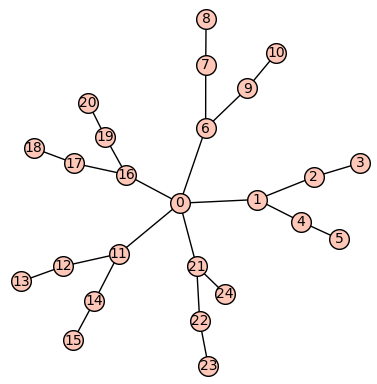
\includegraphics[scale=0.4]{koncni_graf25}
\caption{Graf na 25 vozliščih $wSz = 6686$}
\end{figure}

\begin{figure}[h]
\centering
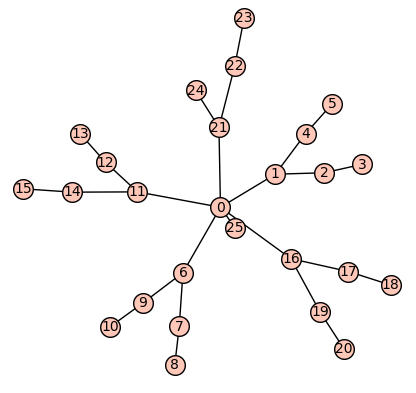
\includegraphics[scale=0.4]{iskanje_graf26}
\caption{Začetni graf na 26 vozliščih $wSz = 7682$}
\end{figure}

\begin{figure}[h]
\centering
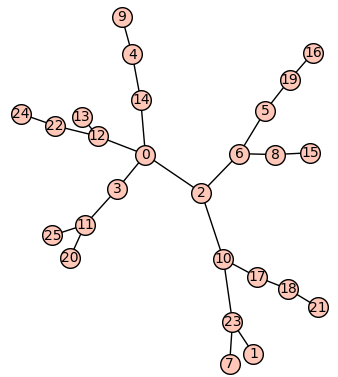
\includegraphics[scale=0.4]{iskanje_graf26_2}
\caption{Graf na 26 vozliščih po 40000 korakih $wSz = 7632$}
\end{figure}

\newpage

\begin{figure}[h]
\centering
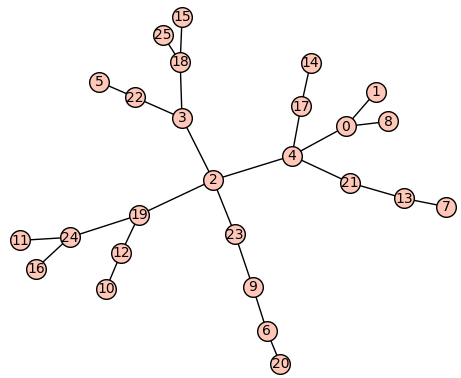
\includegraphics[scale=0.4]{iskanje_graf26_3}
\caption{Graf na 26 vozliščih po 80000 korakih $wSz = 7560$}
\end{figure}

\begin{figure}[h]
\centering
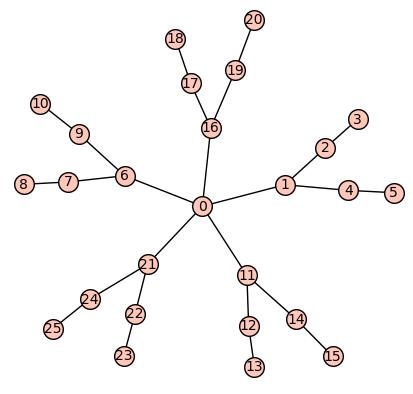
\includegraphics[scale=0.4]{koncni_graf26}
\caption{Graf na 26 vozliščih na koncu $wSz = 7350$}
\end{figure}


Graf na 25 vozliščih je imel vsa poddrevesa iz vozlišča enaka, razen na enem je bilo vozlišče manj. Ravno na tem mestu je na koncu postopka končalo dodatno vozlišče. Tako smo dobili graf z minimalnim $wSz$ na 26 vozliščih, ki ima koren povezan s 5 vozlišči, vsi pa imajo povsem enako strukturo. 




\newpage

\begin{figure}[h]
\centering
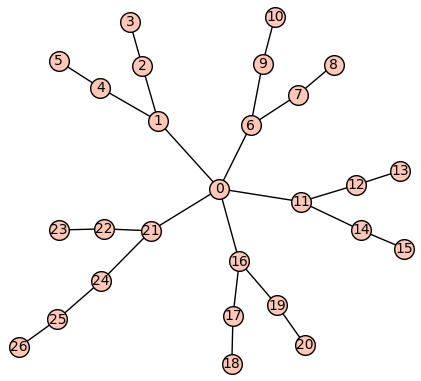
\includegraphics[scale=0.4]{koncni_graf27}
\caption{Graf na 27 vozliščih na koncu $wSz = 8118$}
\end{figure}

\begin{figure}[h]
\centering
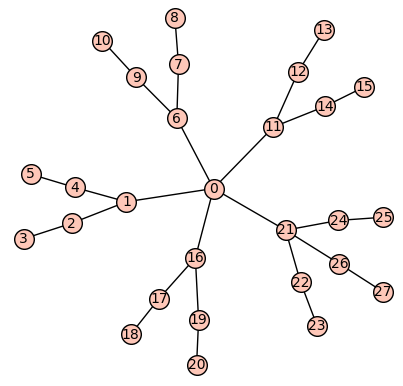
\includegraphics[scale=0.4]{koncni_graf28}
\caption{Graf na 28 vozliščih na koncu $wSz = 8910$}
\end{figure}

\begin{figure}[h]
\centering
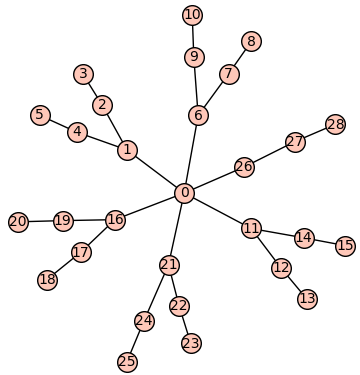
\includegraphics[scale=0.4]{koncni_graf29}
\caption{Graf na 29 vozliščih na koncu $wSz = 9864$}
\end{figure}

Ko dodamo dodatno vozlišče na graf z minimalnim $wSz$ na 28 vozliščih, opazimo, da s povečanjem števila vozlišč na 29 nastane novo poddrevo, ki je povezano direktno s korenom (vozlišče 0).

Končni grafi so bili vedno drevesa, brez ciklov in vedno ena povezava manj od števila vozlišč. Rezultati podpirajo predpostavko, da imajo  minimalni $wSz$ le drevesa.

\newpage

\begin{figure}[h]
\centering
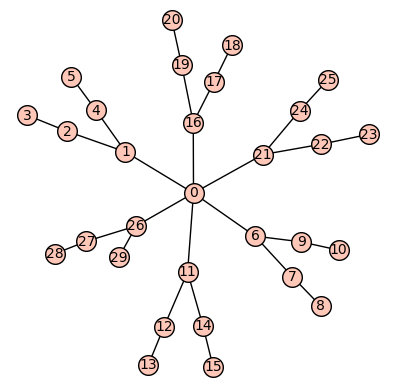
\includegraphics[scale=0.4]{koncni_graf30}
\caption{Graf na 30 vozliščih na koncu $wSz = 10714$}
\end{figure}

\begin{figure}[h]
\centering
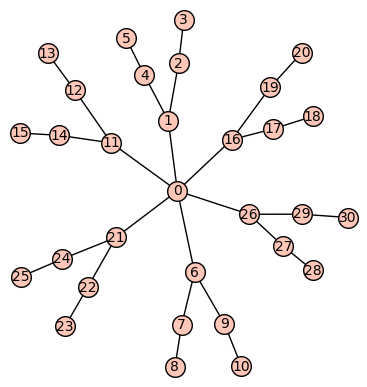
\includegraphics[scale=0.5]{koncni_graf31}
\caption{Graf na 31 vozliščih na koncu $wSz = 11580$}
\end{figure}



\newpage

\section[Lastnosti ekstremnih grafov]{Lastnosti ekstremnih grafov}
\begin{itemize}

\item Za grafe s 7 do 30 vozlišči smo poiskali vrednosti $wSz$ in jih tudi primerjali z vrednostmi iz grafa na ena manj vozlišču.

\begin{table}[!h]
\centering
\caption{Izračunani wSz-ji minimalnih grafov in primerjave s prejšnimi}
\begin{tabularx}{\linewidth}{|*{6}{X|}}
\hline
n & wSz & razlika &  n & wSz & razlika      \\ \hline
  7 & 204& -     & 19 & 3292& 418         \\ \hline
  8 & 306& 102& 20 & 3758&  466      \\ \hline
  9 & 432& 126& 21 & 4240&  482      \\ \hline
10 & 578& 146& 22 & 4806&  566      \\ \hline
11 & 762& 184& 23 & 5396&  590      \\ \hline
12 & 970& 208& 24 & 6038&  642       \\ \hline
13 & 1210& 240& 25 & 6686& 648         \\ \hline
14 & 1476& 266& 26 & 7350& 664        \\ \hline
15 & 1780& 304& 27 & 8118& 768       \\ \hline
16 & 2100& 320& 28 & 8910& 792        \\ \hline
17 & 2472& 372& 29 & 9864& 954         \\ \hline
18 & 2874& 402& 30 & 10714& 850         \\ \hline
\end{tabularx}
\end{table}

\large  \item Struktura grafov

Ob pogledu na samo strukturo grafov hitro vidimo določene podobnosti med grafi ter celo ponavljanja v sami zgradbi grafov. Graf na 26 vozliščih ima namreč koren grafa povezan s petimi vozlišči in prav vsak od teh ima povsem enako strukturo poddrevesa. \\
Graf na 27 vozliščih ima nato dodatno vozlišče na koncu poddrevesa, že pri naslednjem grafu pa vidimo da se dodatna vozlišča v primerjavi z grafom na 26 vozliščih pripneta bližje korenu, ter da ima tako graf na enem vozlišču kaj tri veje z dvema vozliščema. \\
Pri grafu na 29 vozliščih opazimo, da se tri dodatna vozlišča pripnejo direktno na koren grafa, koren je na tem koraku povezan že z šestimi ostalimi vozlišči. \\
Graf na 30 vozliščih ima potem zelo podobno strukturo kot graf na 25 vozliščih, s tem da ima eno dodatno poddrevo s petimi vozlišči. \\
Opazimo torej, da se dodatna vozlišča povezujejo v nova poddrevesa z največ 5 vozlišči, ki je direktno povezano s korenom, ko so vsa poddrevesa enaka se dodatno vozlišče sicer doda na konec lista, tisti podgraf ima nato 6 vozlišč, že v naslednjem koraku pa se to dodatno vozlišče skupaj z novim poveže direktno s korenom in dobimo novo podvejo. 

\newpage

\large  \item  Diameter grafov z minimalnim $wSz$ indeksom\\ \linebreak
Ob podrobnejšem ogledu strukture grafov z vozlišči med 20 in 30 hitro opazimo določene značilnosti in ponavljajoča zaporedja povezav. \\
Diameter oziroma premer grafa je maksimalno število povezav med dvema vozliščema v grafu. \\
Na grafu s $25$ in $26$ vozlišči je ta vrednost enaka $6$. Pri grafu s $27$ vozlišči pa opazimo, da je zaradi podaljšane veje z dodatnim vozliščem premer grafa enak $7$. Že pri naslednjem grafu z $28$ vozlišči ta vrednost zopet pade nazaj na $6$, saj se spremeni struktura grafa. \\
Podobna situacija se zgodi tudi pri grafu s $32$ vozlišči, kjer se dodatno vozlišče zopet doda na konec poddrevesa in je zato vrednost diametra enaka $7$. \\
Z upoštevanjem spreminjanja strukture grafa lahko torej sklepamo, da je diameter grafov enak $6$, razen za grafe z $22 + 5k$ vozlišč. Za grafe z manj kot 20 vozlišč namreč ta sklep ne velja, medtem ko se grafi s premerom $7$ pojavljajo na vsakih 5 grafov.

\end{itemize}
\newpage
\section[Viri]{Viri}

\begin{thebibliography}{9}
\bibitem{research} 
Jan Boka, Boris Furtulab, Nikola Jedličkova in Riste Škrekovski
\textit{On Extremal Graphs of Weighted Szeged Index} 
https://arxiv.org/abs/1901.04764, 15 Jan 2019.

\item \emph{} \url{https://en.wikipedia.org/wiki/Simulated_annealing}, ogled 7.1.2020

\end{thebibliography}


\end{document}